\documentclass{article}
\usepackage[utf8]{inputenc}
\usepackage[margin=1in]{geometry}
\usepackage{amsmath}
\usepackage{amssymb}
\usepackage{tikz}
\usepackage{color}
\usepackage{graphicx}
\usepackage{hyperref}
\usepackage{mathtools}
\usepackage{amsthm}

\title{Torsion Classes and Binary Trees}
\author{Max Weinstein}
\date{December 2019}






\begin{document}


\maketitle

\newtheorem{thm}{Theorem}
\theoremstyle{definition}
\newtheorem{define}[thm]{Definition}


\section{Introduction}
This section will define and give examples of torsion classes and their respective torsion free classes as they appear in relation to other Catalan objects. Furthermore a clear bijection will be given between torsion classes and binary trees. 



\section{Definitions}

\subsection{Torsion Classes}
\begin{define}
A {\it torsion class} is collection of objects in an Abelian category (for our purposes we will only consider the straight categories $\mathcal{A}_n$ with straight orientation) which are closed under extension and quotients. It is useful to think geometrically of the category as being a collection of balls in an equilateral triangle configuration with objects in the torsion class being colored in blue. The property of being closed under extension simply means that if two objects (balls) are in the torsion class, then if a rectangle with vertices at these two dips at most 1 imaginary ball below the bottom of the configuration, the other vertices within the configuration are also in the torsion class.\\
 \end{define}
 \\
\begin{center}
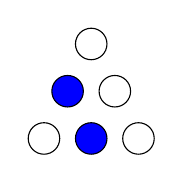
\begin{tikzpicture}
%\draw[help lines=.1] (-4,-4) grid (4,4);

 \draw circle[radius=.2];
 
\begin{scope}[xshift=.6cm]
 \draw[fill=blue] circle[radius=.2];
\end{scope}
 
 \begin{scope}[xshift=1.2cm]
 \draw circle[radius=.2];
\end{scope}

\begin{scope}[xshift=.3cm, yshift=.6cm]
 \draw[fill=blue] circle[radius=.2];
\end{scope}
 
 \begin{scope}[xshift=.9cm, yshift=.6cm]
 \draw circle[radius=.2];
\end{scope}

\begin{scope}[xshift=.6cm, yshift=1.2cm]
 \draw circle[radius=.2];
\end{scope}



\end{tikzpicture}
\end{center}


\subsection{Torsion-Free Class}
\begin{define}
The corresponding {\it torsion-free class} is the collection of balls in the configuration which have the property that there are no homomorphisms from any balls in the torsion class to them. In this case homomorphisms exist if there is a way to draw a complete rectangle within the configuration going up and right from a torsion class ball to another ball. 
\end{define}
We will color objects in the torsion-free class red:
\begin{center}
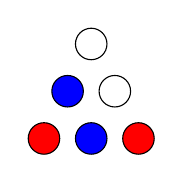
\begin{tikzpicture}
%\draw[help lines=.1] (-4,-4) grid (4,4);

 \draw[fill=red] circle[radius=.2];
 
\begin{scope}[xshift=.6cm]
 \draw[fill=blue] circle[radius=.2];
\end{scope}
 
 \begin{scope}[xshift=1.2cm]
 \draw[fill=red] circle[radius=.2];
\end{scope}

\begin{scope}[xshift=.3cm, yshift=.6cm]
 \draw[fill=blue] circle[radius=.2];
\end{scope}
 
 \begin{scope}[xshift=.9cm, yshift=.6cm]
 \draw circle[radius=.2];
\end{scope}

\begin{scope}[xshift=.6cm, yshift=1.2cm]
 \draw circle[radius=.2];
\end{scope}



\end{tikzpicture}
\end{center}


\subsection{Torsion Pair}
The torsion pair is just a natural algebraic way of describing the torsion class and the corresponding torsion free class simultaneously.
\begin{define}
 A {\it torsion pair} is a pair $(\mathcal{G},\mathcal{F})$ of full subcategories such that:
$$
\mathcal{G}=\{x\,|\, Hom(x,y)=0\, \, \forall y\in \mathcal{F}\}
$$
and 
$$
\mathcal{F}=\{y\, | \, Hom(x,y)=0\, \, \forall x\in \mathcal{G}\}
$$
\end{define}
Where $Hom=0$ means that no rectangle can be drawn from an object $x$ to $y$ where all four vertices are also objects in the category. 

\section{Constructing a Torsion Class}

Torsion classes can be generated by the inclusion of an arbitrary number of objects in the category (If no objects are included this is just the empty torsion class) and by considering in advance the Torsion Pair. Call these objects added $x_n$. Then find the set of all $Y$ such that $Hom(x_n, Y)=0$. $Y$ is the torsion free class. Then find the set of all $X$ such that $Hom(X,Y)=0$ which is the full torsion class. \\
\\
1. Start with an arbitrary selection of objects filled in blue ($x_n$).


\begin{center}
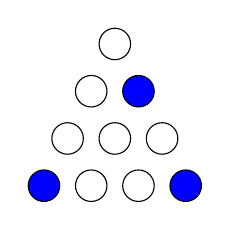
\begin{tikzpicture}
%\draw[help lines=.1] (-4,-4) grid (4,4);

 \draw[fill=blue] circle[radius=.2];
 
\begin{scope}[xshift=.6cm]
 \draw circle[radius=.2];
\end{scope}
 
 \begin{scope}[xshift=1.2cm]
 \draw circle[radius=.2];
\end{scope}

\begin{scope}[xshift=.3cm, yshift=.6cm]
 \draw circle[radius=.2];
\end{scope}
 
 \begin{scope}[xshift=.9cm, yshift=.6cm]
 \draw circle[radius=.2];
\end{scope}

\begin{scope}[xshift=.6cm, yshift=1.2cm]
 \draw circle[radius=.2];
\end{scope}

\begin{scope}[xshift=1.8cm]
 \draw[fill=blue] circle[radius=.2];
\end{scope}

\begin{scope}[xshift=1.5cm, yshift=.6cm]
 \draw circle[radius=.2];
\end{scope}

\begin{scope}[xshift=1.2cm, yshift=1.2cm]
 \draw[fill=blue] circle[radius=.2];
\end{scope}

\begin{scope}[xshift=.9cm, yshift=1.8cm]
 \draw circle[radius=.2];
\end{scope}

\end{tikzpicture}
\end{center}

\noindent 2. Then locate objects where no rectangle can be drawn up/right or down right from a blue object ($Hom=0$) and fill them in red ($Y$). 

\begin{center}
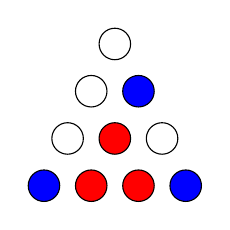
\begin{tikzpicture}
%\draw[help lines=.1] (-4,-4) grid (4,4);

 \draw[fill=blue] circle[radius=.2];
 
\begin{scope}[xshift=.6cm]
 \draw[fill=red] circle[radius=.2];
\end{scope}
 
 \begin{scope}[xshift=1.2cm]
 \draw[fill=red] circle[radius=.2];
\end{scope}

\begin{scope}[xshift=.3cm, yshift=.6cm]
 \draw circle[radius=.2];
\end{scope}
 
 \begin{scope}[xshift=.9cm, yshift=.6cm]
 \draw[fill=red] circle[radius=.2];
\end{scope}

\begin{scope}[xshift=.6cm, yshift=1.2cm]
 \draw circle[radius=.2];
\end{scope}

\begin{scope}[xshift=1.8cm]
 \draw[fill=blue] circle[radius=.2];
\end{scope}

\begin{scope}[xshift=1.5cm, yshift=.6cm]
 \draw circle[radius=.2];
\end{scope}

\begin{scope}[xshift=1.2cm, yshift=1.2cm]
 \draw[fill=blue] circle[radius=.2];
\end{scope}

\begin{scope}[xshift=.9cm, yshift=1.8cm]
 \draw circle[radius=.2];
\end{scope}

\end{tikzpicture}
\end{center}

\noindent 3. Fill in objects blue which have no homomorphism to any red objects. 

\begin{center}
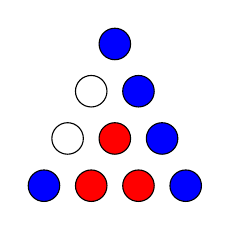
\begin{tikzpicture}
%\draw[help lines=.1] (-4,-4) grid (4,4);

 \draw[fill=blue] circle[radius=.2];
 
\begin{scope}[xshift=.6cm]
 \draw[fill=red] circle[radius=.2];
\end{scope}
 
 \begin{scope}[xshift=1.2cm]
 \draw[fill=red] circle[radius=.2];
\end{scope}

\begin{scope}[xshift=.3cm, yshift=.6cm]
 \draw circle[radius=.2];
\end{scope}
 
 \begin{scope}[xshift=.9cm, yshift=.6cm]
 \draw[fill=red] circle[radius=.2];
\end{scope}

\begin{scope}[xshift=.6cm, yshift=1.2cm]
 \draw circle[radius=.2];
\end{scope}

\begin{scope}[xshift=1.8cm]
 \draw[fill=blue] circle[radius=.2];
\end{scope}

\begin{scope}[xshift=1.5cm, yshift=.6cm]
 \draw[fill=blue] circle[radius=.2];
\end{scope}

\begin{scope}[xshift=1.2cm, yshift=1.2cm]
 \draw[fill=blue] circle[radius=.2];
\end{scope}

\begin{scope}[xshift=.9cm, yshift=1.8cm]
 \draw[fill=blue] circle[radius=.2];
\end{scope}

\end{tikzpicture}
\end{center}

\noindent The total collection of blue objects is the complete torsion class. 


\section{Bijection Between Binary Trees and Torsion Classes}

\subsection{Geometric Correspondence}
For a binary tree with $n$ leaves, take the torsion classes corresponding with triangular configurations of balls having $n-2$ balls along each edge. (i.e. if a binary tree has 5 leaves, take a triangle configuration having 3 balls on each edge). Each ball should be located directly above an "inside leaf" (just a leaf that's not on the end). \\
\\
\begin{center}
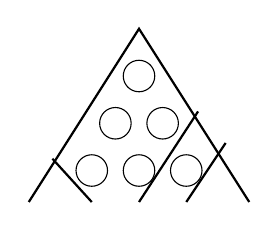
\begin{tikzpicture}

\draw[thick] (-.8,-.4)--(.6, 1.8)--(2,-.4);

\draw[thick] (-.5,.15)--(0,-.4);

\draw[thick] (.6,-.4)--(1.35,.75);

\draw[thick] (1.2,-.4)--(1.7,.35);

 \draw circle[radius=.2];
 
\begin{scope}[xshift=.6cm]
 \draw circle[radius=.2];
\end{scope}
 
 \begin{scope}[xshift=1.2cm]
 \draw circle[radius=.2];
\end{scope}

\begin{scope}[xshift=.3cm, yshift=.6cm]
 \draw circle[radius=.2];
\end{scope}
 
 \begin{scope}[xshift=.9cm, yshift=.6cm]
 \draw circle[radius=.2];
\end{scope}

\begin{scope}[xshift=.6cm, yshift=1.2cm]
 \draw circle[radius=.2];
\end{scope}




\end{tikzpicture}
\end{center}
The bijection is given geometrically like so: Directly above all branches of the binary tree which are descending left to right, color the objects blue. directly above the branches ascending left to right color the objects red. \\
\begin{center}
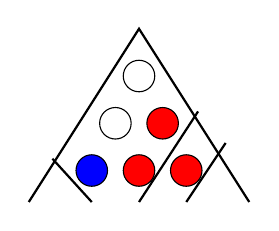
\begin{tikzpicture}

\draw[thick] (-.8,-.4)--(.6, 1.8)--(2,-.4);

\draw[thick] (-.5,.15)--(0,-.4);

\draw[thick] (.6,-.4)--(1.35,.75);

\draw[thick] (1.2,-.4)--(1.7,.35);

 \draw[fill=blue] circle[radius=.2];
 
\begin{scope}[xshift=.6cm]
 \draw[fill=red] circle[radius=.2];
\end{scope}
 
 \begin{scope}[xshift=1.2cm]
 \draw[fill=red] circle[radius=.2];
\end{scope}

\begin{scope}[xshift=.3cm, yshift=.6cm]
 \draw circle[radius=.2];
\end{scope}
 
 \begin{scope}[xshift=.9cm, yshift=.6cm]
 \draw[fill=red] circle[radius=.2];
\end{scope}

\begin{scope}[xshift=.6cm, yshift=1.2cm]
 \draw circle[radius=.2];
\end{scope}




\end{tikzpicture}
\end{center}
\begin{thm}
The collection of objects directly above the descending edges (blue) gives a torsion class and the collection of objects directly above the ascending edges (red) form the corresponding torsion-free class. 

\end{thm}
\noindent {\bf{Proof}} Take our proposed correspondence from binary trees to torsion classes. Above all descending branches should be objects in the torsion class, but why do they form a torsion class? Notice that along descending branches are objects that if one were in the torsion class, they would all have to be, since by our construction of torsion classes objects in the torsion class will fall diagonally below the already included object, since these objects will share the same torsion free objects in common. This is so because there are always homomorphisms between objects on the same diagonal line (so they will never include both torsion and torsion free objects) and because if an object is in the torsion free class with respect to a given torsion object, then an object diagonally downward cannot have any homomorphisms to any of those torsion free objects. Torsion free objects will always be to the left of the descending line or on the bottom row, all of which will not have a homomorphism to objects on the line. Hence we get the descending branches. \\


To go the other direction, from an arrangement of balls draw descending branches underneath objects in the torsion class and ascending branches under objects in the torsion free class. \\
\begin{thm}
The binary tree got from drawing descending branches underneath torsion objects is unique. 
\end{thm}




\\
\noindent {\bf{Proof}} We know that torsion objects give clear instructions for drawing descending branches of binary trees, but how do we know this tree is unique? The proof follows from the fact that binary trees are entirely determined by their descending (or ascending edges). Suppose you fixed the descending edges of a binary tree. Then for all leaves left unconnected, ascending branches must be linked to them, giving the rest of the tree. Since there are only two options for a branch (it is descending or ascending) giving one gives the other since they are complements. It turns out it is always possible to connect all remaining spaces with ascending edges once descending edges are defined. \\
\\

\begin{thm}
The correspondence described above is a bijection.
\end{thm}
\noindent {\bf{Proof}} This follows from the well known fact that there are a Catalan number $C_n$ of both binary trees with $n+1$ leaves and torsion classes with $n-1$ balls in the bottom row. So since a unique tree is given by every torsion class, and a unique torsion class is given by every binary tree, and there are exactly the same number of each, they are in a bijective relationship and the bijection is given by our rule. \\

\\

 
 
 










\end{document}

